\documentclass[11pt,a4paper]{article}
\usepackage[T1]{fontenc}
\usepackage[utf8]{inputenc}
\usepackage{lmodern}
\usepackage[margin=2.5cm]{geometry}
\usepackage{amsmath,amssymb,amsthm}
\usepackage{mathtools}
\usepackage{booktabs}
\usepackage{graphicx}
\usepackage{algorithm}
\usepackage{algpseudocode}
\usepackage{xcolor}
\usepackage{microtype}
\usepackage[hidelinks]{hyperref}
\usepackage{url}

\newtheorem{theorem}{Theorem}
\newtheorem{proposition}[theorem]{Proposition}
\newtheorem{lemma}[theorem]{Lemma}
\newtheorem{corollary}[theorem]{Corollary}
\theoremstyle{definition}
\newtheorem{definition}[theorem]{Definition}
\newtheorem{assumption}{Assumption}
\theoremstyle{remark}
\newtheorem{remark}[theorem]{Remark}

\newcommand{\F}{\mathbb{F}}
\newcommand{\Z}{\mathbb{Z}}
\newcommand{\Q}{\mathbb{Q}}
\newcommand{\End}{\operatorname{End}}
\newcommand{\Tr}{\operatorname{Tr}}
\newcommand{\Nrd}{\operatorname{nrd}}
\newcommand{\Ker}{\operatorname{ker}}
\newcommand{\EA}{E_A}
\newcommand{\EC}{E_C}
\newcommand{\ED}{E_D}
\DeclareUrlCommand\art{\urlstyle{tt}}
\makeatletter\g@addto@macro\UrlBreaks{\do\_\do\-}\makeatother

\setlength{\emergencystretch}{3em}
% Measured and derived numbers used in the text.  Each value cites its record
% in the sentence or table that uses it.  Edit here only.
% Filter acceptance rates (log2 rho) and admissible-degree counts, from
% run-20261011T1955Z-verify/records/f_filter_rate.txt:
%   admissible = log2 f_lo - 1 + log2 rho;  Grover = admissible / 2.
\newcommand{\RhoLOne}{-8.13}
\newcommand{\RhoLThree}{-8.64}
\newcommand{\RhoLFive}{-9.02}
\newcommand{\FspaceLOne}{267.8}
\newcommand{\FspaceLThree}{398.6}
\newcommand{\FspaceLFive}{525.1}
\newcommand{\GroverFLOne}{133.9}
\newcommand{\GroverFLThree}{199.3}
\newcommand{\GroverFLFive}{262.5}
% Decapsulation failure counts (run-20261011T1955Z-verify/records/failrate/):
\newcommand{\FailTotalTrials}{3,635}
\newcommand{\FailRows}{%
Toy16 & 3,005 & 0 & verification run (3,000), benchmark run (5)\\
Toy32 & 603 & 0 & verification run (600), benchmark run (3)\\
L1 & 23 & 0 & verification run (20), benchmark run (3)\\
L3 & 2 & 0 & benchmark run\\
L5 & 2 & 0 & benchmark run\\}
\newcommand{\CTRows}{%
Toy16 & 4 & 2 valid, 1 foreign & 1,116,209,216 in all 12 runs\\
L1 & 2 & key 1: 2 valid, 1 foreign; key 2: 1 valid & 120,996,429,610 in all 4 runs\\}
\newcommand{\DudectT}{$+1.17$ on the raw samples and at most $2.36$ in absolute value after cropping at the 50th, 75th and 90th percentiles}


\title{Eigen-S\'eta: an isogeny KEM whose trapdoor is a hidden-degree endomorphism\\[0.3em]
\large Specification, correctness, heuristic security analysis and a constant-time implementation}
\author{Anonymous}
\date{Revision 2 of 2026-10-17 (first draft 2026-10-11) --- research draft, not peer reviewed}

\begin{document}
\maketitle

\begin{abstract}
We specify Eigen-S\'eta~v2, a key encapsulation mechanism built on supersingular
isogenies in which the decryption trapdoor is a secret endomorphism of the
public curve. The public key is a curve $\EA$ together with an eigenbasis, on
its $2^E$-torsion, of the endomorphism $\tau=\varepsilon\omega\hat\varepsilon$,
where $\omega$ is the degree-2 endomorphism of the curve with complex
multiplication by $\Z[(1+\sqrt{-7})/2]$ and $\varepsilon$ is an isogeny of
\emph{secret} degree $f$. A ciphertext is the codomain of a $3^{F}$-isogeny
together with the images of that eigenbasis under FESTA-style diagonal masks.
The masks commute with the eigen-structure, so the holder of $f$ decodes the
ciphertext with a single $(2^E,2^E)$-isogeny in dimension two (Kani's lemma),
while to anyone else the ciphertext is a masked-torsion isogeny instance.
We give the algorithms, prove correctness (including that the kernel used in
decryption is always cyclic), derive parameters, and analyse key- and
message-recovery attacks. This second revision adds an assessment. We show
that a candidate secret degree can be tested on the public key alone with a
Kani chain of about $2\log_2 f$ steps, half the length of a decapsulation.
We implemented this test: it accepted the true degree and rejected all
\PkWrongTested\ wrong candidates at L1, L3 and L5. It lowers the cost of the
degree search but leaves it far from binding. The binding attack is still
guessing the mask ratio modulo about $\sqrt{3^F}$, at about $2^\lambda$
classical and $2^{\lambda/2}$ Grover queries. We therefore withdraw
revision~1's conjecture of NIST categories 1, 3 and 5 for the sets L1, L3 and
L5 in its unqualified form. Those sets meet the AES references only in NIST's
gate count under MAXDEPTH. At least $2^\lambda$ quantum queries is met only by
L5 (as the level-1 set) and by quantum-hardened sets Q3 and Q5 with
3904- and 5192-bit primes. Both claims assume that the hidden orientation of
$\EA$ cannot be made effective. We identify this as the scheme's largest
risk, because an effective orientation would give subexponential quantum key
recovery at every set. At level~1, public keys and ciphertexts are
1344~bytes. The maintained Rust implementation decapsulates with a theta
chain in about \DecTimeOne\,s on a 4-core cloud VM. The security of the scheme
is a conjecture supported by the analysis in this paper only; it has not
been reviewed by others.
\end{abstract}

\tableofcontents

\section{Introduction}\label{sec:intro}

After the 2022 attacks on SIDH~\cite{CD23,MMPPW23,Rob23}, isogeny-based public-key
encryption needs a trapdoor that does not reveal enough torsion information to
let the attacker run those same attacks. Two families
survive. In the first, torsion images are masked so that the attacker cannot
recover them exactly, as in M-SIDH~\cite{FMP23} and FESTA~\cite{BMP23}; in the
second, the scheme avoids torsion images altogether. FESTA decrypts by running
the torsion attack itself with the help of a secret: the legitimate receiver
knows a matrix that commutes with the masks.

Castryck and Vercauteren~\cite{CV23} observed that a torsion basis which is an
eigenbasis of a \emph{known} endomorphism of small degree makes masked-torsion
instances easy: the masks act diagonally on the eigenvectors, so the
endomorphism's action on the masked points is known exactly, and a lollipop
endomorphism can be decoded with Kani's lemma. They presented this as an
attack, and as a backdoor available to whoever chose the basis.

\paragraph{This work.} Eigen-S\'eta turns that observation into a trapdoor. The
public key is a curve $\EA$ with an eigenbasis of an endomorphism
$\tau\in\End(\EA)$ whose degree $2f^2$ is \emph{secret}. The sender masks the
images of the eigenbasis under a $3^F$-isogeny $\varphi$ with a random diagonal
matrix. The receiver, who knows $f$, knows how
$\theta=\varphi\tau\hat\varphi$ acts on the masked points and recovers $\varphi$
from one $(2^E,2^E)$-isogeny between products of elliptic curves. Without $f$,
the ciphertext is a FESTA-type masked-torsion instance, and the public key is
an isogeny instance of unknown degree from a known curve.

An earlier variant~\cite{EigenSetaNote} took $\tau=\varepsilon\omega\hat\varepsilon$
with $\varepsilon$ of \emph{public} degree $5^k$. That variant is insecure:
its decryption key is a function of the public degree alone
(\S\ref{sec:walk}). Version~2, specified here, draws $f$ from an interval of
about $2^{277}$, $2^{408}$ or $2^{535}$ values, depending on the level, and keeps it secret.

\paragraph{Contributions.}
\begin{itemize}
\item A complete specification of the KEM (\S\ref{sec:scheme}) with the
  Fujisaki--Okamoto transform with implicit rejection~\cite{HHK17}.
\item Proofs that decryption is correct (\S\ref{sec:correctness}). These
  include a proposition that the kernel recovered during decryption is always
  cyclic, which settles a corner case reported for the earlier toy prototype.
\item Parameter sets for $\lambda=128,192,256$ (\S\ref{sec:params}) and a
  heuristic analysis of key recovery, message recovery, quantum attacks,
  chosen-ciphertext attacks and decryption failures (\S\ref{sec:security}).
  The concrete figures are summarised in Table~\ref{tab:attacks}.
\item A Rust implementation with constant-time decapsulation, checked with an
  instruction-count probe and a statistical timing test. The probe found one
  compiler-introduced branch, which we fixed (\S\ref{sec:impl}).
\item Measured sizes, timings and correctness rates at all parameter sets, and
  constant-time evidence at Toy16 and L1 (\S\ref{sec:results}), each
  traceable to a committed record.
\end{itemize}

\paragraph{What this paper does not claim.} Security is a conjecture backed by
the attacks we considered; no third party has analysed the scheme. The
implementation is research code. Its decapsulation is slow, mainly because
the dimension-2 chain is computed in Mumford coordinates; a theta-coordinate
chain~\cite{DMPR23} is future work. Key generation is not constant time.

\paragraph{Evidence conventions.} Each measured number carries the path of the
record it comes from, relative to the root of the repository
(\art{crypto:}). Derived quantities are marked as such.

\section{Preliminaries}\label{sec:prelim}

\paragraph{Curves and isogenies.} Let $p$ be a prime and $\F_{p^2}=\F_p(i)$ with
$i^2=-1$ ($p\equiv3\bmod4$). All curves are supersingular and defined over
$\F_{p^2}$. Isogenies are separable. For an isogeny $\phi$ we write $\hat\phi$
for its dual, so that $\hat\phi\phi=[\deg\phi]$. For $N$ coprime to $p$, the
$N$-torsion $E[N]\cong(\Z/N)^2$ carries the Weil pairing $e_N$, and
$e_N(\phi P,\phi Q)=e_N(P,Q)^{\deg\phi}$.

\paragraph{The base curve.} Let $\ED$ be the curve with $j$-invariant $-3375$.
It has complex multiplication by $\mathcal{O}_K=\Z[(1+\sqrt{-7})/2]$, and it is
supersingular over $\F_p$ whenever $-7$ is not a square modulo $p$, i.e.\
$p\equiv3,5,6\pmod 7$. Its endomorphism $\omega$ of degree~2 satisfies
$\omega^2-t\omega+2=0$ with $t=\pm1$, so $(2\omega-t)^2=-7$. We use the short
Weierstrass model $y^2=x^3-3jkx-2jk^2$ with $j=-3375$ and $k=j-1728$. Since
$p+1=2^{E+1}3^Fc$, every curve in the isogeny class has
$\#E(\F_{p^2})=(p+1)^2$ and full rational $2^E$- and $3^F$-torsion.

\paragraph{Eigenbases.} Let $s_D$ be a square root of $-7$ modulo $2^{E+2}$
(it exists because $-7\equiv1\bmod8$), and set
$\mu=(t+s_D)/2$ and $\nu=(t-s_D)/2$ modulo $2^E$. These are the two roots of
$x^2-tx+2$ modulo $2^E$, and $\mu-\nu=s_D$ is odd. Hence $\omega$ has
eigenvectors $P_D,Q_D$ spanning $\ED[2^E]$ with $\omega P_D=\mu P_D$ and
$\omega Q_D=\nu Q_D$.

\paragraph{Kani's lemma in the form used here.} Let $E$ be a curve, $\gamma\in\End(E)$
and $c'\in\Z$ with $\deg\gamma+c'^2=2^E$. Then
\[
\Phi=\begin{pmatrix} c' & -\hat\gamma\\ \gamma & c'\end{pmatrix}:E^2\to E^2
\]
satisfies $\hat\Phi\Phi=[2^E]$. It is therefore a $(2^E,2^E)$-isogeny between
principally polarised abelian surfaces, and its kernel is
$\{(c'R,-\gamma R):R\in E[2^E]\}$. Given $\gamma(R)$ for a basis of
$E[2^E]$, the isogeny $\Phi$ can be computed as a chain of $E$
$(2,2)$-isogenies~\cite{Kan97,CD23,Rob23}, and it can then be evaluated at
points outside the $2^E$-torsion. In particular $\Phi(X,0)=(c'X,\gamma X)$
reveals $\gamma$ on any subgroup.

\paragraph{$(2,2)$-chains.} A chain from $E\times E$ can pass through
products of elliptic curves (product steps), glue into the Jacobian of a
genus-2 curve, continue with Richelot isogenies, and split back into a
product. We use the gluing, Richelot and splitting formulas of Castryck and
Decru~\cite{CD23} in Mumford coordinates. The order in which these step types
occur is the \emph{schedule} of the chain.

\paragraph{FESTA masking.} In FESTA~\cite{BMP23}, the images of a torsion
basis under a secret isogeny are published multiplied by a secret matrix. We
use diagonal masks: $(a\varphi P,b\varphi Q)$ with odd $a,b$ modulo $2^E$. The
Weil pairing reveals $ab$. The ratio $b/a$ stays hidden.

\section{The scheme}\label{sec:scheme}

\subsection{Parameters}
A parameter set consists of the following data.
\begin{itemize}
\item Exponents $E$ and $F$ and a cofactor $c$ such that
  $p=2^{E+1}3^Fc-1$ is prime and $p\equiv3,5,6\pmod 7$.
\item $d=3^F$, the sender's isogeny degree.
\item A lower bound $f_{\mathrm{lo}}$ for the secret degree, which ranges over
  $[f_{\mathrm{lo}},2f_{\mathrm{lo}})$.
\item The curve $\ED$, its endomorphism $\omega$ with trace $t$, the values
  $s_D,\mu,\nu$ and the eigenbasis $(P_D,Q_D)$ of \S\ref{sec:prelim}.
\item Domain-separated instances of SHAKE256: $G$ (masks), $H_P$ (public-key
  hash), $H_K$ (shared secret) and $H_R$ (rejection key).
\end{itemize}
The concrete sets are in \S\ref{sec:params}.

\paragraph{Canonical bases.} $\textsf{Basis}_3(A)$ deterministically
computes a basis $(P_3,Q_3)$ of $E[3^F]$ on the Montgomery curve
$E:y^2=x^3+Ax^2+x$. It tries $x=1+i,2+i,\dots$, lifts each to a point,
multiplies by $(p+1)/d$, and keeps the first two points whose
$3^{F-1}$-multiples generate $E[3]$. It depends only on $A$, so sender and
receiver agree on it.

\subsection{Key generation}

\begin{algorithm}[h]
\caption[$\textsf{KeyGen}()$]{$\textsf{KeyGen}()$}\label{alg:keygen}
\begin{algorithmic}[1]
\Repeat \Comment{secret degree and Kani scalars}
  \State $f\gets$ uniform odd integer in $[f_{\mathrm{lo}},2f_{\mathrm{lo}})$
  \State reject if $3\mid f$, $7\mid f$ or $2f\equiv 2^E\pmod d$
  \State $m\gets 2^E-7d^2f^2$; find $c,c'$ with $c^2+c'^2=m$, $c$ even, or reject
  \State $s_0\gets f s_D \bmod 2^E$
  \State choose signs of $c,c'$ with $\max(v_2(c'-\lambda_S),v_2(c'+\lambda_S))=2$, where $\lambda_S=ds_0+c$, or reject
\Until{accepted}
\State $g\gets 2^E-f$
\Repeat \Comment{endomorphism of norm $fg$ that uses Frobenius}
  \State pick $(y_0,y_1)\ne(0,0)$ with $T\gets fg-p\,N(y_0+y_1\omega)>0$ prime, $T\equiv1,2,4\pmod7$
  \State solve $x^2+7y'^2=T$ (Cornacchia); $x_0\gets x-ty'$, $x_1\gets 2y'$
\Until{found}
\State $\alpha\gets x_0+x_1\omega+(y_0+y_1\omega)\pi$ \Comment{$\pi$ the $p$-Frobenius; $\Nrd\alpha=fg$}
\State compute the $(2^E,2^E)$-isogeny with kernel $\{([f]R,\alpha R):R\in\ED[2^E]\}$; reject unless its first step is a gluing
\State from its codomain $E_1\times E_2$, pick the factor $\EA$ whose map $\varepsilon:\ED\to\EA$ has degree $f$ (test $e(\varepsilon X,\varepsilon Y)=e(X,Y)^f$ on $\ED[3^F]$)
\State $\lambda_1,\lambda_2\gets$ uniform odd residues modulo $2^E$
\State $P_A\gets\lambda_1\varepsilon(P_D)$, $Q_A\gets\lambda_2\varepsilon(Q_D)$; bring $\EA$ to Montgomery form $y^2=x^3+Ax^2+x$
\State $\lambda_T\gets c-ds_0$; reject if $\lambda_S,\lambda_T$ or $c'\equiv-1\pmod{2^E}$, or $c$ or $c'\equiv-1\pmod d$
\State $\mathit{pk}\gets(A,x(P_A),x(Q_A),x(P_A-Q_A))$; \ $z\gets$ 32 random bytes
\State $\mathit{sk}\gets(\lambda_S,\lambda_T,c'\bmod 2^E,c\bmod d,c'\bmod d,z,\mathit{pk})$
\State \Return $(\mathit{pk},\mathit{sk})$ after a self-test encapsulation and decapsulation
\end{algorithmic}
\end{algorithm}

The degree-$f$ factor $\varepsilon$ exists by Kani's lemma applied to
$\alpha$, since $\deg\alpha+f^2=f\cdot2^E$ and $\gcd(f,g)=1$
(see~\cite[\S2]{Rob23}). The requirement $(y_0,y_1)\ne(0,0)$ excludes
$\alpha\in\Z[\omega]$, for which $\EA$ would lie in the small orbit of $\ED$
under the class group of $\mathcal{O}_K$ (\S\ref{sec:weak}). The
endomorphism the public key is built around is
\[
\tau=\varepsilon\omega\hat\varepsilon\in\End(\EA),\qquad \deg\tau=2f^2,\quad \Tr\tau=tf,
\]
and since $\tau\varepsilon=f\,\varepsilon\omega$, the points
$P_A,Q_A$ are eigenvectors of $\tau$ on $\EA[2^E]$ with eigenvalues $f\mu$ and
$f\nu$. The scalars $\lambda_1,\lambda_2$ make the Weil pairing
$e(P_A,Q_A)=e(P_D,Q_D)^{\lambda_1\lambda_2 f}$ uniform among
values of the same order, so it carries no information on $f$.

\subsection{Encapsulation}

\begin{algorithm}[h]
\caption[$\textsf{Encaps}(\mathit{pk})$ and the deterministic core $\textsf{Enc}(\mathit{pk},s)$]{$\textsf{Encaps}(\mathit{pk})$ and the deterministic core $\textsf{Enc}(\mathit{pk},s)$}\label{alg:encaps}
\begin{algorithmic}[1]
\State $s\gets$ uniform in $\Z/d$; \ $\mathit{ct}\gets\textsf{Enc}(\mathit{pk},s)$; \ \Return $(\mathit{ct},\,H_K(s,\mathit{ct}))$
\Statex
\Function{Enc}{$\mathit{pk}=(A,x_P,x_Q,x_{P-Q}),s$}
  \State $(P_3,Q_3)\gets\textsf{Basis}_3(A)$; \ $K\gets P_3+sQ_3$ \Comment{3-point ladder}
  \State $\varphi:\EA\to\EC=\EA/\langle K\rangle$ \Comment{chain of $F$ 3-isogenies, fixed strategy}
  \State push $x_P,x_Q,x_{P-Q}$ through $\varphi$: $P'=\varphi(P_A)$, $Q'=\varphi(Q_A)$
  \State $(a,b)\gets G(s,H_P(\mathit{pk}))$, odd residues modulo $2^E$
  \State \Return $(A_C,\ x(aP'),\ x(bQ'),\ x(aP'-bQ'))$
\EndFunction
\end{algorithmic}
\end{algorithm}

\subsection{Decapsulation}

Write $S=aP'$ and $T=bQ'$, and
$\theta=\varphi\tau\hat\varphi\in\End(\EC)$. Section~\ref{sec:correctness}
shows that $\psi=2\theta-tdf$ has degree $7d^2f^2$ and trace~0, and acts on
$S$ and $T$ by $\pm ds_0$. Decapsulation applies Kani's lemma to
$\gamma=\psi+c$, whose degree is $7d^2f^2+c^2=2^E-c'^2$.

\begin{algorithm}[h]
\caption[$\textsf{Decaps}(\mathit{sk},\mathit{ct})$]{$\textsf{Decaps}(\mathit{sk},\mathit{ct})$}\label{alg:decaps}
\begin{algorithmic}[1]
\State parse $\mathit{ct}=(A_C,x_S,x_T,x_{S-T})$; lift $S,T$ on $\EC$ with $x(S-T)=x_{S-T}$; on failure \Return $H_R(z,\mathit{ct})$ \Comment{public}
\State $(X_1,X_2)\gets\textsf{Basis}_3(A_C)$; \ $(P_3,Q_3)\gets\textsf{Basis}_3(A)$ \Comment{public}
\State $\Phi\gets$ the $(2^E,2^E)$-isogeny of $\EC^2$ with kernel $\langle(c'S,-\lambda_SS),(c'T,-\lambda_TT)\rangle$, fixed schedule
\State evaluate $\Phi$ at $(X_1,0),(0,X_1),(X_2,0)$; identify both codomain factors with $\EC$ among the $8$ sign and order choices by comparing with $c'X_i$; read off $\gamma(X_1),\gamma(X_2)$
\State $\psi(X_i)\gets\gamma(X_i)-cX_i$ for $i=1,2$
\State $G\gets$ whichever of $\psi(X_1),\psi(X_2)$ has order $d$; $H\gets$ the other; find $k$ with $H=kG$ \Comment{pairings, DLP in $\mu_d$}
\State $\hat\varphi\gets\EC/\langle X_h-kX_g\rangle\to\EA$; \ $K_g\gets$ the image of $X_1$ or $X_2$ that has order $d$
\State $s\gets\log(e(P_3,K_g))/\log(e(K_g,Q_3))$ in $\mu_d$
\State $\mathit{ct}'\gets\textsf{Enc}(\mathit{pk},s)$
\State \Return $H_K(s,\mathit{ct})$ if $\mathit{ct}'=\mathit{ct}$, else $H_R(z,\mathit{ct})$ \Comment{constant-time selection}
\end{algorithmic}
\end{algorithm}

All steps after line~2 run in constant time with respect to $\mathit{sk}$ and
$s$ (\S\ref{sec:impl}). Lines~1--2 depend only on public data.

\subsection{The transform}
$\textsf{Enc}$ is a deterministic public-key encryption of the message
$s\in\Z/d$, derandomised by deriving the masks from $G(s,H_P(\mathit{pk}))$.
The KEM is the $U^{\not\perp}$ transform with implicit rejection of Hofheinz,
H\"ovelmanns and Kiltz~\cite{HHK17} applied to it. The re-encryption check
compares the entire ciphertext, including the curve coefficient.

\section{Correctness}\label{sec:correctness}

Throughout, $(\mathit{pk},\mathit{sk})$ is honestly generated,
$\mathit{ct}=\textsf{Enc}(\mathit{pk},s)$, and the notation of
Algorithms~\ref{alg:keygen}--\ref{alg:decaps} is in force. Write
$\theta=\varphi\tau\hat\varphi\in\End(\EC)$ and $\psi=2\theta-tdf$.

\begin{lemma}[the lollipop endomorphism]\label{lem:psi}
$\Tr\psi=0$ and $\deg\psi=7d^2f^2$. Moreover $\psi S=ds_0S$ and
$\psi T=-ds_0T$, where $s_0=fs_D\bmod 2^E$.
\end{lemma}

\begin{proof}
$\Tr\theta=\varphi(\tau+\hat\tau)\hat\varphi=\varphi[tf]\hat\varphi=tdf$, and
$\deg\theta=d^2\deg\tau=2d^2f^2$. Hence $\Tr\psi=2\Tr\theta-2tdf=0$ and
\[
\deg\psi=(2\theta-tdf)(2\hat\theta-tdf)=4\deg\theta-2tdf\Tr\theta+t^2d^2f^2=8d^2f^2-2d^2f^2+d^2f^2=7d^2f^2 .
\]
For the eigenvalues, $\hat\varphi S=a\hat\varphi\varphi P_A=adP_A$, and
$\tau P_A=f\mu P_A$, so $\theta S=adf\mu\,\varphi P_A=df\mu S$. Likewise
$\theta T=df\nu T$. Then $\psi S=df(2\mu-t)S=dfs_DS$, and
$\psi T=df(2\nu-t)T=-dfs_DT$.
\end{proof}

The masks $a,b$ drop out because $S$ and $T$ are multiples of eigenvectors.
This is where the trapdoor is used: only $f$ (through $s_0$) and the Kani
scalars are needed, never $\varphi$ or the masks.

\begin{proposition}[the decryption isogeny]\label{prop:kani}
Let $\gamma=\psi+c$. Then $\deg\gamma+c'^2=2^E$, and the subgroup
$\langle(c'S,-\lambda_SS),(c'T,-\lambda_TT)\rangle$ of $\EC^2$ is the kernel of
the $(2^E,2^E)$-isogeny $\Phi=\begin{psmallmatrix}c'&-\hat\gamma\\ \gamma&c'\end{psmallmatrix}$.
\end{proposition}

\begin{proof}
$\deg\gamma=\deg\psi+c\Tr\psi+c^2=7d^2f^2+c^2=2^E-c'^2$ by the choice of
$c,c'$. By Lemma~\ref{lem:psi}, $\gamma S=(ds_0+c)S=\lambda_SS$ and
$\gamma T=(c-ds_0)T=\lambda_TT$. The points $S,T$ form a basis of $\EC[2^E]$,
because $\varphi$ has odd degree and $a,b$ are odd. So the two generators
are $(c'R,-\gamma R)$ for $R=S,T$, and the kernel statement is Kani's lemma
(\S\ref{sec:prelim}).
\end{proof}

From $\Phi(X,0)=(c'X,\gamma X)$, decapsulation obtains $\gamma$, and hence
$\psi=\gamma-c$, on $\EC[d]$. Restricted to $\EC[d]$ we have
$\psi=2\varphi\tau\hat\varphi$, since $d\mid tdf$.

\begin{proposition}[the recovered kernel is always cyclic]\label{prop:cyclic}
$\psi(\EC[d])$ is cyclic of order $d$, and the kernel of $\psi$ restricted to
$\EC[d]$ is exactly $\ker\hat\varphi$.
\end{proposition}

\begin{proof}
We have $\hat\varphi(\EC[d])=\ker\varphi=\langle K\rangle$, which is cyclic of
order $d$. The endomorphism $\tau$ has degree $2f^2$, which is prime to $3$,
so $\tau\langle K\rangle$ is again cyclic of order $d$. The map $\varphi$ is
injective on $\tau\langle K\rangle$ if and only if
$\tau\langle K\rangle\cap\langle K\rangle=0$, i.e.\ if and only if the two
subgroups have different subgroups of order~$3$. That fails only if the line
$L=\langle 3^{F-1}K\rangle\subset\EA[3]$ is an eigenline of $\tau$ modulo~3.
The characteristic polynomial of $\tau$ is $x^2-tfx+2f^2$, whose
discriminant is $f^2(t^2-8)=-7f^2\equiv 2f^2\pmod 3$. Since $3\nmid f$, this is
a non-square modulo~3. So $\tau$ has no eigenline in $\EA[3]$, and $\varphi$
maps $\tau\langle K\rangle$ isomorphically onto a cyclic group of order $d$.
Thus $\psi(\EC[d])=2\varphi\tau\langle K\rangle$ has order $d$, its kernel
has order $d^2/d=d$, and that kernel contains $\ker\hat\varphi$, which also
has order~$d$.
\end{proof}

\begin{remark}\label{rem:noncyclic}
The design note~\cite{EigenSetaNote} reported a ``non-cyclic $\psi'$'' corner
case in one of eight trials of its toy prototype, a variant with a different
$\psi'$ and very small $d=3^5$. Proposition~\ref{prop:cyclic} shows that the
case cannot occur in version~2. The argument needs only that $-7$ is a
non-square modulo~3 and $3\nmid\deg\tau$. The cause of the toy observation
was not isolated.
\end{remark}

\begin{proposition}[recovery of $s$]\label{prop:s}
Let $G$ be a generator of $\psi(\EC[d])$ and $H=kG$ the image of the other
basis point. Then $\ker\hat\varphi=\langle X_h-kX_g\rangle$. If $K_g$ is the image
under $\hat\varphi$ of a basis point and has order $d$, then $K_g=u(P_3+sQ_3)$
for a unit $u$, and
$s=\log e(P_3,K_g)/\log e(K_g,Q_3)$ in $\mu_d$.
\end{proposition}

\begin{proof}
$\psi(X_h-kX_g)=H-kG=0$, and $X_h-kX_g$ has order $d$, so by
Proposition~\ref{prop:cyclic} it generates $\ker\hat\varphi$. The image of
$\EC[d]$ under $\hat\varphi$ is $\ker\varphi=\langle P_3+sQ_3\rangle$. With
$\zeta=e(P_3,Q_3)$, which has order $d$, we get $e(K_g,Q_3)=\zeta^u$ and
$e(P_3,K_g)=\zeta^{us}$. The codomain of $\hat\varphi$ is $\EA$ up to
isomorphism, and isomorphisms preserve these subgroups. The implementation
maps the codomain to the model with coefficient $A$, using $x\mapsto-x$ when
the computed coefficient is $-A$.
\end{proof}

\begin{proposition}[fixed schedule]\label{prop:schedule}
In the basis $(S,0),(T,0),(0,S),(0,T)$ of $\EC^2[2^E]$, the coordinates of
$\ker\Phi$ are the columns of
$\begin{psmallmatrix}c'&0\\0&c'\\-\lambda_S&0\\0&-\lambda_T\end{psmallmatrix}$
modulo $2^E$, which depend on $\mathit{sk}$ only. Whether each $(2,2)$-step of
the chain is a product step, a gluing, a Richelot step or a splitting is
decided by linear conditions on these coordinates modulo powers of~2. So the
schedule is the same for every ciphertext under a given key.
\end{proposition}

\begin{proof}[Proof sketch]
The kernel of the $j$-th step is $2^{E-j}$ times the image of $\ker\Phi$ under
the first $j-1$ steps. On a product $E_1\times E_2$, the step is a product
step exactly when its 2-torsion kernel is a direct product
$\langle(P,0),(0,Q)\rangle$, and a graph step when it is the graph of the
identity of $\EC[2]$ (on $\EC\times\EC$) or of an isomorphism (after the
split). Both are statements about the coordinates. On a Jacobian, the step
is a splitting exactly when the codomain is a product, which happens at a
fixed index determined by the same 2-adic data. Key generation imposes
$\max(v_2(c'\mp\lambda_S))=2$ and the gluing test of line~15, which fixes the
schedule as graph, product, glue, Richelot${}^{E-6}$, split, product, graph.
The self-test checks it once.
\end{proof}

\paragraph{Correctness error.} By the propositions above, decapsulation of an
honest ciphertext returns $H_K(s,\mathit{ct})$ unless an intermediate formula
meets a degenerate input. Examples are a Mumford divisor not in general
position, a zero denominator in a Richelot or splitting formula, or a Miller
line through the second argument. No branch handles these cases. The output
is then wrong but computed in the same time, and the FO check rejects it.
Heuristically each such event has probability $O(1/p)$ per step, giving
$\delta=O(E/p)\approx2^{-1330}$ at level~1. Key generation excludes the one
structured degenerate case, a scalar $\equiv-1$ modulo the point order, which
the x-only ladder with $y$-recovery cannot handle. The measured rates are in
Table~\ref{tab:failures}: no failure occurred in \FailTotalTrials\
decapsulations.

\section{Parameters}\label{sec:params}

The parameter sets are produced by \art{crypto:eigen_seta/examples/gen_params.rs},
which writes \art{crypto:eigen_seta/src/params_generated.rs}. They satisfy
four constraints.
\begin{enumerate}
\item[(P1)] $d=3^F\ge 2^{2\lambda}$, with $F=\lceil 2\lambda/\log_2 3\rceil$.
  Message recovery costs about $\sqrt d$ (\S\ref{sec:msg}).
\item[(P2)] $2^E>28\,d^2f_{\max}^2$ with $f_{\max}=2f_{\mathrm{lo}}$. Then
  $m=2^E-7d^2f^2>\tfrac34 2^E$ for every admissible $f$, so the two-squares
  step has a large target. $E$ is the smallest exponent that works.
\item[(P3)] $f_{\mathrm{lo}}=2^\kappa\lfloor p/2^E\rfloor+1$. Then
  $fg\gtrsim 2^\kappa p$, and the norm equation $N(x)+pN(y)=fg$ has about
  $2^\kappa$ candidate values of $y\ne0$. We take $\kappa=12$ for the real sets
  and $\kappa=8$ for the toys.
\item[(P4)] $p=2^{E+1}3^Fc-1$ is prime with $p\equiv3,5,6\pmod7$, and $c$ is the
  smallest cofactor that achieves this.
\end{enumerate}

Since $f\approx 2^{\kappa+1}cd$ and $2^E\approx 28d^2f^2$, we get
$p\approx 2^{E+1}d\approx d^5\cdot 2^{2\kappa+O(1)}c^2$. That is
$\log_2p\approx 10\lambda$. The factor $d^5$ is the price of decrypting with
a single chain, whose torsion order must exceed the degree $7d^2f^2+c^2$ of
$\gamma$. Evaluating $\Phi$ from two half-chains, as in SQIsign~2D-style
implementations~\cite{DMPR23}, would let $2^E$ shrink to about
$\sqrt{\deg\gamma}$. We have not implemented this.

\begin{table}[h]
\centering
\caption[Parameter sets]{Parameter sets. $d=3^F$; ``$f$ bits'' is the bit length of the secret
degree in the recorded keys; public key and ciphertext are four
$\F_{p^2}$ elements each. Source:
\art{crypto:eigen_seta/src/params_generated.rs}; $f$ bits from
\art{crypto:research/eigen_seta_rust_20261011/reports/run-20261011T1813Z-bench/records/bench_output.txt}.}
\label{tab:params}
\begin{tabular}{lrrrrrrrrr}
\toprule
set & $\lambda$ & $\log_2 p$ & $E$ & $F$ & $\log_2 d$ & $c$ & $\kappa$ & $f$ bits & pk = ct (B)\\
\midrule
Toy16 & 16 & 216 & 174 & 21 & 33.3 & 158 & 8 & 51 & 216\\
Toy32 & 32 & 369 & 297 & 41 & 65.0 & 55 & 8 & 80 & 376\\
L1 & 128 & 1341 & 1076 & 162 & 256.8 & 144 & 12 & 278 & 1344\\
L3 & 192 & 1991 & 1594 & 243 & 385.1 & 1059 & 12 & 409 & 1992\\
L5 & 256 & 2630 & 2106 & 324 & 513.5 & 380 & 12 & 536 & 2632\\
\bottomrule
\end{tabular}
\end{table}

The toy sets have no security; they exist so that every code path can be
tested quickly.

\section{Security analysis}\label{sec:security}

This section is heuristic. We state the problems the scheme relies on,
reduce key recovery to finding $f$, and estimate the cost of every attack we
know of. Table~\ref{tab:attacks} summarises the estimates. A cost written
$2^x\cdot C$ means $2^x$ evaluations of a polynomial-time subroutine $C$,
typically a $(2,2)$-chain in dimension~2 or an isogeny chain in dimension~8.

\subsection{Problems}

\begin{assumption}[hidden-degree eigenbasis problem]\label{ass:key}
Given the public parameters and $\mathit{pk}=(\EA,P_A,Q_A)$, it is hard to
find $f$, or any secret key that decapsulates honest ciphertexts for
$\mathit{pk}$.
\end{assumption}

\begin{assumption}[masked eigen-torsion problem]\label{ass:msg}
Given $\mathit{pk}$ and $\mathit{ct}=\textsf{Enc}(\mathit{pk},s)$ for uniform
$s\in\Z/d$, it is hard to find $s$. This is the one-wayness of the
deterministic PKE inside the KEM.
\end{assumption}

\begin{lemma}[the degree is the key]\label{lem:fiskey}
Given $f$, a working secret key can be computed in polynomial time, up to a
choice among the few representations of $m=2^E-7d^2f^2$ as a sum of two
squares.
\end{lemma}

\begin{proof}
$s_0=fs_D$ is public once $f$ is known. The pair $(c,c')$ is one of the
representations $c^2+c'^2=m$; key generation finds one with the same
procedure an attacker would use, and the schedule condition and the signs
leave at most a handful of candidates. Each candidate can be tested by
decapsulating a self-made ciphertext. Neither $\alpha$, $\varepsilon$ nor
$\lambda_1,\lambda_2$ is needed.
\end{proof}

So Assumption~\ref{ass:key} is equivalent to the hardness of finding $f$. A
consequence is that $\EA$ and the eigen-structure must hide $f$; the next
subsection shows what goes wrong when they do not.

\subsection{The public-degree variant is insecure}\label{sec:walk}

The toy prototype of~\cite{EigenSetaNote} had a ``walk'' variant: $\EA$ was
the codomain of a secret isogeny $\varepsilon$ of \emph{public} degree $5^k$,
and $\tau=\varepsilon\omega\hat\varepsilon$. Its decryption key
$(c,c',s_0)$ is computed from $\Delta'=4\deg\tau-(\Tr\tau)^2=7\cdot25^k$ and
from nothing else, as the merged code shows
(\art{crypto:research/eigen_seta_prototype_20261011/eigen_seta_toy.py},
lines 133--155 and 201--202). Since $k$ is public, anyone can compute the key
and decrypt. An exploratory run, not archived, decrypted 5 of 5 toy
ciphertexts this way. Version~2 exists to close this hole: the degree of
$\tau$ is $2f^2$ with $f$ secret.

\subsection{Key recovery}\label{sec:key}

\paragraph{Exhaustive search over $f$.} An attacker can enumerate candidates
$f$, apply key generation's public filters, derive a candidate key by
Lemma~\ref{lem:fiskey}, and test it with one decapsulation. The filters
accept a fraction $\rho$ of the odd candidates in $[f_{\mathrm{lo}},2f_{\mathrm{lo}})$.
We measured $\rho$ empirically
(\art{crypto:research/eigen_seta_rust_20261011/reports/run-20261011T1955Z-verify/records/f_filter_rate.txt}):
$\log_2\rho=\RhoLOne$, $\RhoLThree$ and $\RhoLFive$ at L1, L3 and L5 (measured from 200, 100 and 100 accepted candidates, so about $\pm0.1$ to $\pm0.14$ binomial standard error). This
leaves about $2^{\FspaceLOne}$, $2^{\FspaceLThree}$ and $2^{\FspaceLFive}$
admissible degrees, an upper bound since the later rejections of key
generation are not counted. The search costs that many chain evaluations
classically and their square root with Grover's algorithm. We know of no
test that rejects a wrong $f$ more cheaply than a full chain. In the toy
experiment of~\cite[\S6]{EigenSetaNote}, 85 of 86 wrong but
pairing-consistent guesses, including guesses agreeing with the truth on
3--13 low bits, ran the whole chain and failed only at the final split
(\art{crypto:research/eigen_seta_prototype_20261011/results/}).

\paragraph{Recovering $\varepsilon$ from a path.} Let $I$ be any left
$\End(\ED)$-ideal connecting $\ED$ to $\EA$. The isogeny $\varepsilon$
corresponds to an equivalent ideal of norm $f$. There are about
$\tfrac{15}{2\pi^2}X^2$ cyclic isogenies of degree at most $X$ from $\ED$,
spread over about $p/12$ curves, so on average about $9X^2/p$ of them land
on a given curve. For $X=2f_{\mathrm{lo}}$ this is about $2^{-782}$ at
level~1. So $\varepsilon$
is, with overwhelming probability, the unique shortest isogeny from $\ED$ to
$\EA$, and a reduced basis of $I$ yields it, and $f$, in polynomial time.
Key recovery therefore costs no more than finding \emph{some} isogeny from
$\ED$ to $\EA$. That is the supersingular path or endomorphism-ring
problem~\cite{EHLMP18,Wes22}: $\tilde O(p^{1/2})$ classically~\cite{DG16}
and $\tilde O(p^{1/4})$ quantumly~\cite{BJS14}. We also list $p^{1/3}$ as a
conservative classical figure in view of recent heuristic algorithms with
large memory~\cite[\S1.1]{EigenSetaNote}. Because $p\approx d^5$, all three
are far beyond the target.

\paragraph{Meet in the middle on $\varepsilon$.} If $f$ is smooth, $\varepsilon$
factors and a meet-in-the-middle search becomes possible. Even with $f$
known and perfectly balanced, it costs at least $\sqrt f\ge\sqrt{f_{\mathrm{lo}}}$:
$2^{138.5}$, $2^{204.1}$ and $2^{267.5}$ at the three levels, which is above
$2^\lambda$, and it applies only to the fraction of keys with smooth $f$.

\paragraph{Torsion-point attacks on the public key.} The public key reveals
$\varepsilon$ on $\ED[2^E]$, with $2^{2E}\gg f$, up to the diagonal scalars
$\lambda_1,\lambda_2$. The SIDH attacks~\cite{CD23,MMPPW23,Rob23} need the
degree to build the auxiliary isogeny of degree $2^E-f$ or $N^2-f$. With $f$
unknown they reduce to the exhaustive search above. Hiding the degree as a
countermeasure to these attacks also appears in terSIDH and
binSIDH~\cite{BF23}, where the secret degree ranges over products of small
prime powers; here it ranges over an interval. Knowing $f$ would make
$\lambda_1,\lambda_2$ irrelevant: $\tau$ acts on $(P_A,Q_A)$ as
$f\cdot\mathrm{diag}(\mu,\nu)$ whatever the scaling, and the attacker could
simply decrypt.

\paragraph{Leakage through the public key.} The Weil pairing
$e(P_A,Q_A)=e(P_D,Q_D)^{\lambda_1\lambda_2f}$ is uniform among primitive
$2^E$-th roots of unity, because $\lambda_1\lambda_2$ is a uniform unit.
The eigenvalues of $\tau$ are $f\mu$ and $f\nu$, with $\mu,\nu$ public, so an
attacker knows the action of $\tau$ on $\EA[2^E]$ up to the unknown scalar
$f\bmod 2^E$. We do not know how to use this without $f$. The decryption
identity $\deg\gamma+c'^2=2^E$ involves $f^2$ through $\deg\tau$, so there is
no smaller Kani instance that tests $f$ modulo $2^j$. This is the main
structural assumption of the scheme, and it is where we would look first for
an attack.

\subsection{Message recovery}\label{sec:msg}

\paragraph{Mask guessing plus a torsion attack (binding).} The ciphertext
contains $S=a\varphi P_A$ and $T=b\varphi Q_A$, with $\varphi$ of public
degree $d$. The pairing $e(S,T)=e(P_A,Q_A)^{abd}$ reveals $ab$, but the
ratio $r=b/a$ is uniform. If $r\bmod 2^n$ were known, the attacker would hold
$\varphi$ on $\EA[2^n]$ up to the common scalar $a$. Robert's attack in
dimension~8~\cite{Rob23} then recovers $\varphi$ in polynomial time as soon
as $2^{2n}>d$. With $r$ odd, guessing it costs $2^{n-1}$ trials,
where $n=\lfloor(\log_2d)/2\rfloor+1$. That is about $2^{128}$, $2^{192}$ and
$2^{256}$ dimension-8 chains classically, and the square root of that with Grover.
FESTA's analysis~\cite{BMP23} rests on the same estimate. An attacker who
knew $\tau$ could do better: the masks act diagonally on eigenvectors of
$\theta=\varphi\tau\hat\varphi$, which is exactly what decapsulation
exploits. But knowing $\tau$ means knowing $f$.

\paragraph{Claw finding on $\varphi$.} Both ends of $\varphi$ are public and
its degree is $d$. A generic meet in the middle costs about $\sqrt d$ time
and memory classically. Tani's algorithm costs $d^{1/3}$ quantum time with
as much quantum memory, but under realistic cost models it was not better
than classical van Oorschot--Wiener search~\cite{vOW99} for SIKE~\cite{JS19}. Our $d$ is
$2^{256.8}$, $2^{385.1}$ and $2^{513.5}$, which exceeds the degrees
$2^{216}$, $2^{305}$ and $2^{372}$ of SIKEp434, p610 and p751~\cite{SIKE}.
Those were assessed against the same attack for categories 1, 3 and 5. So
claw finding is not the binding attack.

\paragraph{Eigenbases of known endomorphisms.} The Castryck--Vercauteren
attacks on FESTA and M-SIDH~\cite{CV23} need an endomorphism of $\EA$ of
small degree for which $(P_A,Q_A)$ is an eigenbasis. The only such
endomorphisms we know are those in $\Z[\tau]$, of degree at least $2f^2$,
and they are not available without $f$.

\subsection{Quantum security and NIST categories}\label{sec:nist}
NIST defines categories 1, 3 and 5 by the cost of key search on AES-128, -192
and -256~\cite{NIST16}. Quantumly, that is Grover search over $2^{128}$,
$2^{192}$ or $2^{256}$ keys with an AES circuit as the oracle. The binding
attack above has the same shape: a Grover search over about $2^{\lambda}$
candidates, but with an oracle (an isogeny chain in dimension~8 over a
1341- to 2630-bit field) that is far more expensive than an AES evaluation.
Classically it is about $2^\lambda$ such chains against $2^\lambda$ AES
evaluations. We therefore \emph{conjecture} that L1, L3 and L5 meet
categories 1, 3 and 5. Two caveats apply. The margin rests on the oracle
cost alone: the search space matches the AES key space and is not larger.
And any attack that guesses less than $\sqrt d$ of mask information would
break the claim.

\subsection{Chosen-ciphertext security and decryption failures}\label{sec:cca}
The KEM is $U^{\not\perp}[\textsf{Enc},G]$~\cite{HHK17}. In the random-oracle
model it is IND-CCA secure if $\textsf{Enc}$ is one-way
(Assumption~\ref{ass:msg}) and has negligible correctness error $\delta$;
quantum random-oracle bounds for implicit rejection also
exist~\cite{BHHHP19}. The adaptive key-recovery attacks that broke static
SIDH keys~\cite{GPST16} send malformed ciphertexts and watch the result.
Here every ciphertext that differs from $\textsf{Enc}(\mathit{pk},s)$ for the
recovered $s$ yields the pseudorandom $H_R(z,\mathit{ct})$, in constant time
(\S\ref{sec:impl}). Decapsulation must also never fail \emph{observably} on
malformed inputs. The robustness test (\S\ref{sec:results}) feeds 48
adversarial ciphertexts, including singular and special curves,
small-order points and random curves: none causes a panic, and none yields
the honest key. Degenerate formula inputs do not give an attacker a failure oracle either.
A crafted ciphertext is answered with $H_R(z,\mathit{ct})$ whether or not
an intermediate formula degenerates, because either way the re-encryption
differs. Only the failure of an \emph{honest} ciphertext would be visible,
as a mismatch with the encapsulated key. That has probability
heuristically $O(E/p)$ (\S\ref{sec:correctness}), and it did not occur in
\FailTotalTrials\ decapsulations. So decryption-failure attacks have nothing
to work with.

\subsection{Weak keys}\label{sec:weak}
\begin{itemize}
\item $\alpha\in\Z[\omega]$, i.e.\ $y=0$. The Kani factor would then be an
  $\mathcal{O}_K$-ideal isogeny, and since $h(-7)=1$ its codomain is $\ED$
  itself (or its conjugate). Key generation forces $(y_0,y_1)\ne(0,0)$.
\item $f\equiv g\pmod d$. The pairing test could not tell the two Kani
  factors apart, so key generation rejects these $f$ via $2f\not\equiv2^E$.
\item Scalars $\equiv-1$ modulo the point order. These break $y$-recovery in
  the ladder; key generation rejects them.
\item The schedule condition and the gluing test. These fix the 2-adic shape
  of $(c',\lambda_S,\lambda_T)$ for all keys. They are public by design, and
  their cost in key entropy is included in $\rho$.
\end{itemize}

\begin{table}[t]
\centering
\caption[Estimated attack costs, as $\log_2$ of the number of basic
operations]{Estimated attack costs, as $\log_2$ of the number of basic
operations. ``chain'' means one isogeny-chain evaluation. All figures are
derived from the parameters, except $\rho$, which is measured. Source of
$\rho$:
\art{crypto:research/eigen_seta_rust_20261011/reports/run-20261011T1955Z-verify/records/f_filter_rate.txt}.}
\label{tab:attacks}
\small
\begin{tabular}{llrrr}
\toprule
target & attack & L1 & L3 & L5\\
\midrule
key & search over admissible $f$, classical (chains) & \FspaceLOne & \FspaceLThree & \FspaceLFive\\
key & same with Grover (chains) & \GroverFLOne & \GroverFLThree & \GroverFLFive\\
key & path to $\EA$ then shortest ideal, classical $p^{1/2}$ / $p^{1/3}$ & 670 / 447 & 995 / 663 & 1315 / 876\\
key & path to $\EA$ then shortest ideal, quantum $p^{1/4}$ & 335 & 498 & 657\\
key & meet in the middle on $\varepsilon$ ($\sqrt f$) & 138.5 & 204.1 & 267.5\\
message & mask guess $+$ dim-8 attack, classical (chains) & 128 & 192 & 256\\
message & same with Grover (chains) & 64 & 96 & 128\\
message & claw on $\varphi$, classical $\sqrt d$ & 128.4 & 192.6 & 256.8\\
message & claw on $\varphi$, quantum $d^{1/3}$ (with $d^{1/3}$ qubits) & 85.6 & 128.4 & 171.2\\
\midrule
\multicolumn{2}{l}{target $\lambda$ (classical) / NIST category} & 128 / 1 & 192 / 3 & 256 / 5\\
\bottomrule
\end{tabular}
\end{table}

\section{Implementation and side channels}\label{sec:impl}

Revision~1 described the Rust crate \art{crypto:eigen_seta/} (about 4,300
lines plus tests), and \S\ref{sec:impl}--\S\ref{sec:results} still describe
and measure that historical build unless they say otherwise. The maintained
implementation is now the sibling repository \art{eigenx:}~\cite{EigenX}.
\S\ref{sec:impl-v2} lists what changed. The crate is generic over the limb
count, so one code base serves all parameter sets. Variable-time big integers (\texttt{num-bigint}) appear only
in key generation and in public constants.

\subsection{Arithmetic}
\begin{itemize}
\item \emph{$\F_p$.} Montgomery multiplication. For our primes $p+1\equiv0
  \bmod 2^{64Z}$, where $Z$ is 16, 24 and 32 limbs out of 21, 32 and 42, so the
  reduction skips the zero limbs of $p+1$ (``Montgomery-friendly'' primes) and
  costs $N(N-Z)$ instead of $N^2$ word products.
\item \emph{Inversion.} Bernstein--Yang safegcd~\cite{BY19}, generalising the
  structure of libsecp256k1's \texttt{modinv64} to any limb count, with the
  proven divstep bound. It is 40 to 140 times faster than Fermat inversion
  at L1--L5 (Table~\ref{tab:field}).
\item \emph{$\F_{p^2}$.} Karatsuba multiplication, inversion via the norm,
  and the constant-time square root of Adj and Rodr\'iguez-Henr\'iquez~\cite{AR14}.
\item \emph{Curves and isogenies.} x-only Montgomery ladders, including a
  three-point ladder, with Okeya--Sakurai $y$-recovery~\cite{OS01}; SIDH-style
  3-isogeny chains with optimal strategies~\cite{CLN16}; Weierstrass
  arithmetic with constant-time selection between the doubling and addition
  formulas; and the gluing, Richelot and splitting maps of~\cite{CD23} in
  Mumford coordinates, with batched inversions. The Weil pairing uses a
  projective Miller loop over the public bits of $3^F$. Discrete logarithms in
  $\mu_{3^F}$ are computed digit by digit with constant-time comparisons.
\end{itemize}

\subsection{Constant-time decapsulation}
Decapsulation is split into two functions so that each can be checked
separately.
\begin{itemize}
\item \texttt{decaps\_prepare} depends only on $(\mathit{pk},\mathit{ct})$.
  It parses both, lifts $S$ and $T$, and computes both canonical bases. It
  runs in variable time.
\item \texttt{decaps\_core} contains everything secret: the Kani chain with
  its fixed schedule, the identification over the 8 sign and order choices,
  the pairings and DLPs, the 3-isogeny chain, the re-encryption, and the
  selection.
\end{itemize}
In the core, no branch and no memory index depends on secret data, and all
loop counts are public. Selections use \texttt{subtle}'s constant-time
primitives, and every mask passes through \texttt{core::hint::black\_box}.
Scalars have fixed widths. Secret scalars and secret byte buffers are wiped on
drop. The only loop whose trip count depends on data, the canonical-basis
search, runs on public curves and is capped. A crafted public key or
ciphertext makes it return a refusal rather than spin.

\paragraph{A compiler-introduced leak.} The masks in safegcd's final
normalisation (add $m$ if negative, negate if requested) are computed
arithmetically, as \texttt{r + (m \& mask)}. LLVM compiled the add into a
conditional that skipped the work when the mask was zero, so the instruction
count depended on the sign of a secret-dependent intermediate. That leak
affected every field inversion. The source had no branch. The
instruction-count probe of \S\ref{sec:results} found it, and annotating the
probe at line level located it. Passing the masks through
\texttt{black\_box} fixed it. This is a reminder that constant-time code must
be checked on the binary.

\subsection{Residual issues}
\begin{itemize}
\item Key generation is variable time: rejection sampling, Cornacchia and
  primality tests. It must run where no attacker can time it.
\item Allocation: the core allocates vectors whose sizes are fixed by the
  parameter set. glibc's allocator then executes a number of instructions
  that depends on the heap state left by earlier variable-time work, though
  not on secrets. A production implementation should use fixed buffers.
\item Points and field elements on the stack are not wiped, only scalars and
  byte buffers.
\item The memory-address side of constant time is argued, not measured: there
  are no secret-indexed tables. Power, EM and fault attacks are out of scope.
  The FO check catches faults that corrupt $s$, but not faults that skip the
  check.
\item Constant time is verified for one compiler (rustc~1.97, release
  profile) and one target (x86-64). Other builds need the probe re-run.
\end{itemize}

\subsection{Tests}
The crate's tests compare the field arithmetic with a big-integer reference
at 1, 2, 9, 21 and 42 limbs, the chain with direct endomorphism evaluation,
and the pairing with bilinearity. They also run round trips at Toy16 and
Toy32. Known-answer tests pin SHA3-256 digests of the public key, ciphertext
and shared secret produced from fixed seeds at Toy16, Toy32 and L1. The
robustness tests feed decapsulation 48 adversarial ciphertexts
(\S\ref{sec:cca}) and encapsulation 14 adversarial public keys; every call
terminates without a panic. A
regression test covers a key-generation hang that we fixed: Tonelli--Shanks
accepted $z=0$ as a non-residue.

\subsection{The maintained implementation (revision 2)}\label{sec:impl-v2}
The following changes in \art{eigenx:} matter for this paper.
\begin{itemize}
\item \emph{Theta-coordinate decapsulation.} The $(2^E,2^E)$-chain of
  decapsulation is a level-2 theta chain ported from Theta-Rust
  (Dartois--Maino--Pope--Robert~\cite{DMPR23};
  \art{eigenx:src/theta.rs}, \art{eigenx:src/chain.rs}). The Mumford chain of
  \S\ref{sec:impl} is kept for variable-time chain inspection only. The
  identification of $\gamma$ on $\EC[d]$ now matches $x$-coordinates per image
  and selects in constant time among the $y$-sign patterns.
\item \emph{Parameters.} The Q3 and Q5 sets, the NUMS prime search of (P4),
  and parallel key-generation attempts. The toy sets are no longer shipped.
\item \emph{Cryptanalysis code.} A cost model (\art{eigenx:src/security.rs})
  and runnable attacks (\art{eigenx:src/cryptanalysis/}): key derivation from
  $f$, the near-miss experiment, meet in the middle on $\varphi$,
  mask-guess/Kani scaffolding, and the public-key degree test of
  Lemma~\ref{lem:pktest} (new in this revision).
\item \emph{A field-arithmetic defect, fixed in this revision.} The
  interleaved products \texttt{Fp::mul2} and \texttt{Fp::mul3}, which
  $\F_{p^2}$ multiplication and squaring use, always took the
  Montgomery-friendly reduction. For a modulus with $p+1\not\equiv0\bmod2^{64}$
  they returned wrong products. The test \texttt{f1} of
  \art{eigenx:tests/field.rs}, on the field of $2^{61}-1$, failed on every run
  on the main branch and passes after the fix
  (\art{crypto:research/eigen_seta_assessment_20261017/records/}). Every Eigen-S\'eta prime
  is Montgomery-friendly, so no parameter set was affected. The fix routes
  other moduli to the generic product, as single multiplication already did.
\end{itemize}
Constant-time evidence (\S\ref{sec:results}) was produced on the historical
Mumford build and has not been repeated on the theta build;
\art{eigenx:SIDE_CHANNELS.md} is the author's assessment of the current code.


\section{Measurements}\label{sec:results}

\S\ref{sec:pktest-results} holds the measurements of revision~2. Everything
before it is the historical measurement of revision~1, made on the
\art{crypto:eigen_seta/} build with the Mumford decapsulation chain. Those
numbers do not describe the maintained theta build.

All historical measurements were taken on one host: an Intel Xeon at 2.80\,GHz (shared
cloud VM, 4 logical cores), using rustc~1.97.0 in release mode. Two runs are
used. The benchmark run \art{run-20261011T1813Z-bench} used the code at
commit \art{19c641d12}. The verification run \art{run-20261011T1955Z-verify}
used commit \art{d504af28e}, which adds the key-generation checks and the
buffer wiping. The later commit \art{72051ac67} only caps the public
canonical-basis search; the known-answer tests confirm that it changes no
output. Their records are under
\art{crypto:research/eigen_seta_rust_20261011/reports/}.

\subsection{Sizes and speed}

\begin{table}[h]
\centering
\caption[Wall time per operation on one thread, as the range over trials
(trial count in brackets)]{Wall time per operation on one thread, as the range over trials
(trial count in brackets). Every decapsulation returned the encapsulated key.
Record: \art{run-20261011T1813Z-bench/records/bench_output.txt}.}
\label{tab:timings}
\begin{tabular}{lrrrr}
\toprule
set & pk = ct (B) & keygen (s) & encaps (s) & decaps (s)\\
\midrule
Toy16 & 216 & 0.38 [1] & 0.005--0.008 [5] & 0.12--0.19 [5]\\
Toy32 & 376 & 2.3 [1] & 0.009--0.012 [3] & 0.45--0.59 [3]\\
L1 & 1344 & 32.3 [1] & 0.24--0.26 [3] & 13.4--15.0 [3]\\
L3 & 1992 & 118.6 [1] & 1.03 [2] & 51.8--53.9 [2]\\
L5 & 2632 & 271.8 [1] & 2.17--2.20 [2] & 120.2--124.0 [2]\\
\bottomrule
\end{tabular}
\end{table}

\begin{figure}[h]
\centering
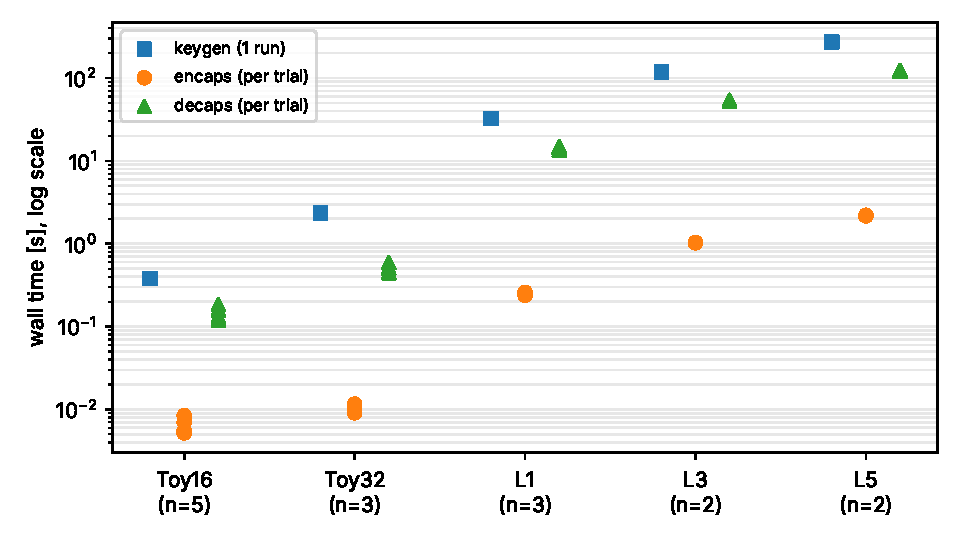
\includegraphics[width=0.78\textwidth]{figures/kem_times.pdf}
\caption[Wall time per operation, every trial shown, log scale]{Wall time per operation, every trial shown, log scale. Measured;
record as in Table~\ref{tab:timings}.}
\label{fig:times}
\end{figure}

Encapsulation is fast because it is a 3-isogeny chain of length $F$.
Decapsulation is dominated by the $E-6$ Richelot steps in Mumford
coordinates. Each step inverts a polynomial modulo a quartic for every point
it moves; from the formulas, we estimate a few hundred $\F_{p^2}$
multiplications per point and step. Key generation is a single sample, and
its time varies widely with the number of rejected candidates.

\begin{table}[h]
\centering
\caption[$\F_p$ arithmetic in ns per operation, in the same binary and run]{$\F_p$ arithmetic in ns per operation, in the same binary and run.
Multiplication is the minimum over 15 repetitions; inversion is the mean of
200. Record: \art{run-20261011T1813Z-bench/records/bench_output.txt}.}
\label{tab:field}
\begin{tabular}{lrrrr}
\toprule
set & limbs & mul & inversion, Fermat & inversion, safegcd\\
\midrule
Toy16 & 4 & 54 & 18,403 & 4,741\\
Toy32 & 6 & 72 & 67,657 & 10,316\\
L1 & 21 & 611 & 1,426,022 & 35,608\\
L3 & 32 & 1,516 & 6,708,390 & 109,506\\
L5 & 42 & 2,449 & 13,453,052 & 96,327\\
\bottomrule
\end{tabular}
\end{table}

No pre-change binary was kept as a baseline for the KEM-level timings, so we
claim no KEM-level speedup from the field optimisations.

\subsection{Correctness}

\begin{table}[h]
\centering
\caption[Decapsulation outcomes for honest ciphertexts with fresh OsRng keys
and ciphertexts]{Decapsulation outcomes for honest ciphertexts with fresh OsRng keys
and ciphertexts. Records:
\art{run-20261011T1955Z-verify/records/failrate/}, plus the benchmark run.}
\label{tab:failures}
\begin{tabular}{lrrl}
\toprule
set & trials & failures & record\\
\midrule
\FailRows
\bottomrule
\end{tabular}
\end{table}

Zero failures in 3,005 trials bounds the failure rate at Toy16 only by
about $10^{-3}$ at 95\% confidence (rule of three). The argument that the
rate is negligible is the heuristic $O(E/p)$ of \S\ref{sec:correctness};
the trials show that no systematic failure mode exists.

Beyond these, the known-answer tests and the robustness tests pass: 48
adversarial ciphertexts to decapsulation and 14 adversarial public keys to
encapsulation, with no panic and no hang (\art{crypto:eigen_seta/tests/}).

\subsection{Constant-time evidence}

Callgrind counted the instructions executed by \texttt{decaps\_core} alone,
with keys and ciphertexts generated from fixed seeds
(\art{crypto:eigen_seta/examples/ct_probe.rs}). The count splits into glibc's
allocator and \texttt{mem*} routines, whose work depends on heap layout but
not on secrets (\S\ref{sec:impl}), and everything else.

\begin{table}[h]
\centering
\caption[Instructions executed in the secret phase of decapsulation,
excluding glibc's allocator]{Instructions executed in the secret phase of decapsulation,
excluding glibc's allocator. ``Foreign'' ciphertexts are well formed but made
for another key, so the FO check rejects them. Records:
\art{run-20261011T1955Z-verify/records/toyprobe/ctprobe_summary.txt} and
\art{.../l1probe/ctprobe_summary.txt}.}
\label{tab:ct}
\begin{tabular}{lllr}
\toprule
set & keys & ciphertexts per key & non-allocator instructions\\
\midrule
\CTRows
\bottomrule
\end{tabular}
\end{table}

\begin{figure}[h]
\centering
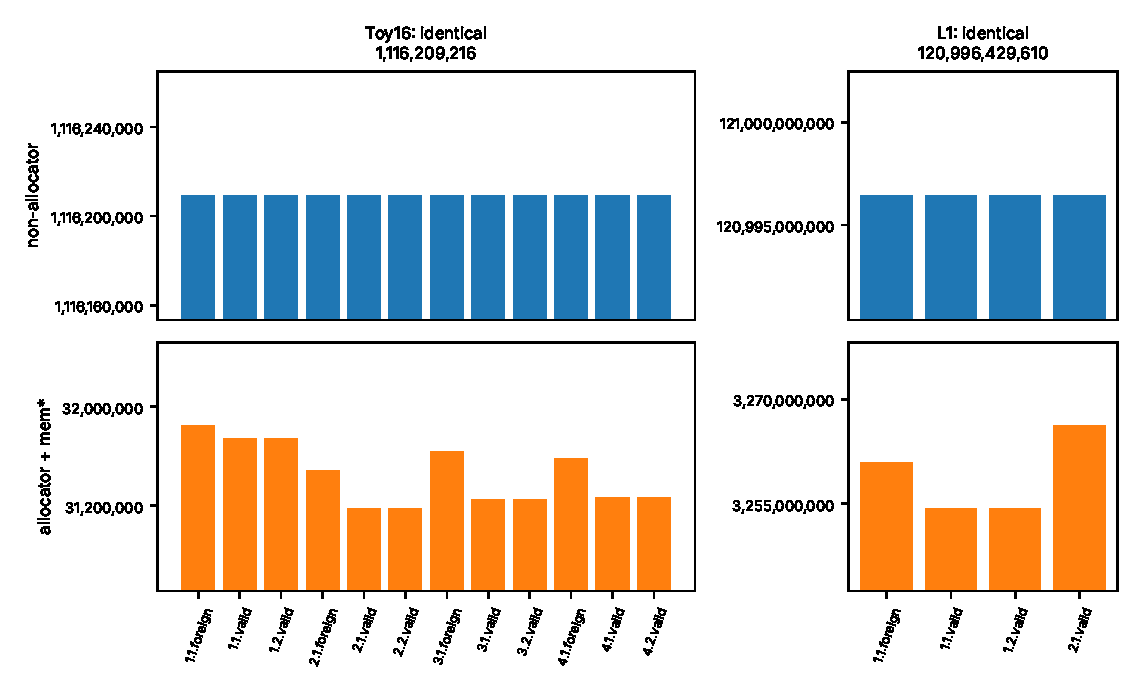
\includegraphics[width=0.78\textwidth]{figures/ct_probe.pdf}
\caption[Instruction counts of \texttt{decaps\_core} per run, at Toy16 (12
runs) and L1 (4 runs)]{Instruction counts of \texttt{decaps\_core} per run, at Toy16 (12
runs) and L1 (4 runs). Top: everything except glibc's allocator. Bottom:
glibc's allocator and \texttt{mem*}. Measured; records as in
Table~\ref{tab:ct}.}
\label{fig:ct}
\end{figure}

A statistical timing test in the style of dudect~\cite{RBV17}
(\art{crypto:eigen_seta/examples/dudect_decaps.rs}) used one Toy16 key and
interleaved two classes in random order: a fixed ciphertext and a pool of 16
fresh ones, half of them FO-rejected. With 1,000 samples per class, Welch's
statistic was \DudectT. The usual threshold for a detected leak is
$|t|>4.5$. This test is weaker than the instruction counts: it uses one key,
wall-clock time on a shared VM, and compares ciphertext classes rather than
keys. Record: \art{run-20261011T1955Z-verify/records/dudect_output.txt}.

\subsection{Revision 2: the public-key degree test}\label{sec:pktest-results}
Run \art{run-20261017T1623Z-pk-degree-test} executed
\art{eigenx:examples/pk_degree_test.rs} at \art{eigenx} commit
\art{94fe2d9} on a shared cloud VM (Intel Xeon at 2.10\,GHz, 4 logical
cores, rustc~1.97.0, release build, no core pinning). Records:
\art{crypto:research/eigen_seta_assessment_20261017/records/run-20261017T1623Z-pk-degree-test/}. For each
set it generates one key with its true $f$ and tests the true degree and a
number of wrong candidates with the theta chain of Lemma~\ref{lem:pktest}. A
candidate is accepted when the codomain is $\EA$. The wrong candidates are
uniform odd values prime to 21 and near misses $f+j2^k$ with
$k\in\{16,64,\lfloor\tfrac12\log_2f\rfloor\}$, $j\le4$. At L1 the true degree
and one wrong candidate were also walked with the structural checks of the
Mumford inspector. The true degree glued, ran all $e-6$ Richelot steps and
split exactly at the end. The wrong one glued, ran all steps with no early
split, and did not split.

\begin{table}[h]
\centering
\caption[Public-key degree test]{Public-key degree test. $e$ is the chain
length for the true degree, $e_{\min}=\lfloor\log_2 7f^2\rfloor+2$ is the shortest length the planner tries, and ``excess''
is the mean of $e-e_{\min}$ over the wrong candidates. The timings are the
median and range over interleaved repetitions of one test and one full
decapsulation of an honest ciphertext under the same key, wall time with
the crate's internal threads. Measured; record as above.}
\label{tab:pktest}
\small
\resizebox{\textwidth}{!}{%
\begin{tabular}{lrrrrrrr}
\toprule
set & $E$ & $e$ (true $f$) & $e_{\min}$ & excess & wrong (accepted) & test (s) & decaps (s)\\
\midrule
\PkRows
\bottomrule
\end{tabular}}
\end{table}

\begin{figure}[h]
\centering
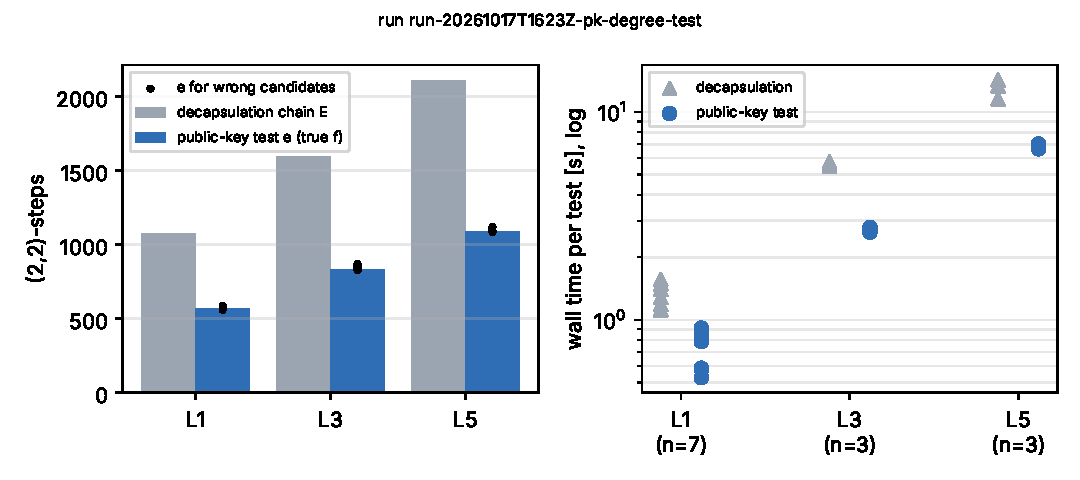
\includegraphics[width=0.78\textwidth]{figures/pk_test.pdf}
\caption[Public-key degree test against decapsulation]{Chain length (left)
and wall time per test (right) of the public-key degree test and of
decapsulation, every repetition shown. Measured; run \art{run-20261017T1623Z-pk-degree-test}.}
\label{fig:pktest}
\end{figure}

The chain is $e/E\approx0.52$ of the decapsulation chain at every set,
because $e\approx2\log_2f$ and $E\approx4\log_2f$. The ratio of the median
times is 1.6 at L1 and 2.0 at L3 and L5. Decapsulation also pays for
ladders, pairings and the re-encryption. The L1 ranges overlap less
cleanly, and we do not explain the lower ratio there. These timings are on a noisy shared
VM and support only the factor-of-two reading. The cost model's gate
columns for the degree search drop by $1.9$ bits as a result. This changes
no tier, because the degree search is far from binding.


\section{Assessment (revision 2)}\label{sec:assessment}

This section records an assessment of the scheme made on 2026-10-17 against
the maintained implementation~\cite{EigenX}. It is still the authors' own
analysis, not an external review. Its method was as follows. We recomputed
every derived number in Tables~\ref{tab:params}, \ref{tab:attacks} and
\ref{tab:tiers} from the parameters and the cost model, and reread the
proofs of \S\ref{sec:correctness}. We read the key-generation filter that
defines the degree search space. We ran the maintained test suite. We
implemented and measured one new attack component, the test of
Lemma~\ref{lem:pktest}. Records:
\art{crypto:research/eigen_seta_assessment_20261017/}.

\paragraph{Verdict.} We found no attack below the costs of
Table~\ref{tab:attacks}. The binding attack is still mask guessing, at about
$2^\lambda$ classical chains and $2^{\lambda/2}$ Grover queries on the L sets
and $2^\lambda$ queries on L5, Q3 and Q5. Security rests on two assumptions
that have no reduction to a standard problem. Assumption~\ref{ass:key} is that
the hidden-degree eigenbasis with its hidden orientation hides $f$.
Assumption~\ref{ass:msg} is that the masked eigen-torsion problem is hard, and
IND-CPA needs its decisional form. We rank the risks as follows.
\begin{enumerate}
\item \emph{An effective orientation of $\EA$.} The public key is a segment
  of length $2E$ of a horizontal $2$-walk in the hidden
  $\Z[f\omega]$-orientation. Any method that extends this to an evaluable
  class-group action gives subexponential quantum key recovery through
  Kuperberg's algorithm. It does so at every parameter set, because the Q sets
  enlarge $d$ and not $f$. The level-structure
  frameworks~\cite{DFP24,Arpin24} and sesquilinear pairings are the tools to
  check first. Nobody has done that.
\item \emph{A mask-free higher-dimensional embedding.} The subgroups
  $\varphi\langle P_A\rangle$ and $\varphi\langle Q_A\rangle$ and the product
  $ab$ are public and do not depend on the mask ratio. A Kani embedding of
  dimension~4 or~8 built from them alone would remove the binding attack's
  $\sqrt d$ search. This is open.
\item \emph{The decisional assumption.} Every basis of $\EA[2^E]$ is an
  eigenbasis of some endomorphism, so the assumption is about the size of the
  smallest diagonal one. No distinguisher is known, and no argument for
  hardness is known beyond the absence of one.
\end{enumerate}

\paragraph{Corrections to revision 1.}
\begin{itemize}
\item \emph{NIST categories} (relabelling, claim correction). Revision~1
  conjectured categories 1, 3 and 5 for L1, L3 and L5 on the strength of
  AES-like structure. That holds only in the gate-count metric (Tier A of
  \S\ref{sec:nist}). Against $2^\lambda$ quantum queries (Tier B), L1 and L3
  fall short at $2^{64.5}$ and $2^{96.5}$. Only L5, Q3 and Q5 meet that bar.
\item \emph{The degree-search oracle} (advance in the attack's cost
  accounting, small). A candidate degree can be tested on the public key
  alone with a chain of about $2\log_2f$ steps instead of a decapsulation
  of $E\approx4\log_2f$ steps (Lemma~\ref{lem:pktest},
  \S\ref{sec:pktest-results}). This lowers the degree-search row by about
  1.9 bits in the gate model. It changes no tier.
\item \emph{Implementation and measurements} (engineering). The paper now
  points to the maintained code, which decapsulates with a theta chain and
  adds the Q sets. Revision~1's timings and constant-time evidence describe
  the historical Mumford build only (\S\ref{sec:impl-v2}). A field-arithmetic
  defect for non-friendly moduli was found and fixed. It affected no
  parameter set.
\item \emph{Two inconsistencies in the maintained security notes}
  (documentation). \art{eigenx:docs/SECURITY.md} placed the public
  $\omega$-eigenbasis on $\ED[3^F]$. That is impossible, because $3$ is inert
  in $\Q(\sqrt{-7})$, and Proposition~\ref{prop:cyclic} rests on there being
  no eigenline modulo~3. The note is corrected. Its cost model takes the
  admissible fraction of degrees to be $1/\ln2^E$ and says this is the
  density of sums of two squares. Key generation actually accepts $f$ when
  $2^E-7d^2f^2$, after removing prime factors up to $2^{14}$, leaves 1 or a
  prime $\equiv1\pmod4$, together with the divisibility and sign conditions of Algorithm~\ref{alg:keygen}. The measured rate $\rho$
  (\S\ref{sec:key}) is the right quantity. It exceeds the model's fraction
  by 1.6 to 2.3 bits, so the model understates the search, which is the
  conservative direction.
\end{itemize}

\paragraph{Practicality.} Primes of about $10.5\lambda$ bits (1341 bits at
L1, 3904 and 5192 bits for Q3 and Q5) make public keys and ciphertexts 1.3 to
5.2\,kB. Key generation is a rejection search that takes hours at Q5 even
with eight workers (\art{eigenx:research/q5_roundtrip.md}). The decryption
chain is the cost driver. Shortening it with two half-chains (open
problem~3) would bring $p$ from about $d^5$ to about $d^3$, and it is the
most valuable engineering change.

\section{Open problems}\label{sec:conclusion}

\begin{enumerate}
\item \emph{Cryptanalysis of the hidden degree.} The scheme stands or falls
  with the claim that the public key gives no handle on $f$ beyond
  exhaustive search (\S\ref{sec:key}). In particular, the attacker knows the
  action of $\tau$ on $\EA[2^E]$ up to the scalar $f\bmod 2^E$. Independent
  analysis of this point is the most important next step.
\item \emph{Mask entropy.} The binding attack guesses $b/a$ modulo about
  $\sqrt d$. Any way to use fewer torsion bits, for example a dimension-4
  variant of the torsion attack, or a lollipop built from another known
  endomorphism, would lower the security level directly.
\item \emph{Smaller primes.} Decrypting with two half-chains would shrink
  $2^E$ from about $7d^2f^2$ to its square root and cut $p$ from about $d^5$ to
  about $d^3$, by the derivation of \S\ref{sec:params} with $2^{2E}>\deg\gamma$.
\item \emph{Speed.} Theta-coordinate $(2,2)$-chains~\cite{DMPR23} instead of
  Mumford coordinates, stack-only buffers, and SIMD field arithmetic.
\item \emph{Constant-time key generation}, in particular a constant-time
  norm-equation solver.
\item \emph{Compression} of public keys and ciphertexts, by encoding the
  points relative to canonical bases as in compressed SIDH.
\end{enumerate}


\bibliographystyle{alpha}
\bibliography{refs}
\end{document}
